\section{Respuesta en frecuencia}
La ganancia de voltaje y la fase de amplificadores acoplados capacitivamente se
ven afectados cuando la frecuencia de señal se encuentra por debajo de un valor
crítico. En bajas frecuencias, la reactancia de los capacitores de acoplamiento
se vuelve significativa, lo que reduce la ganancia de voltaje e incrementa el
desfasamiento \cite{Floyd}.

\subsection{BJT}

\subsubsection{Calculo de los capacitores del amplificador}
Para hallar los valores de cada capacitor del amplificador anterior sección se
calculan los siguientes valores:

\begin{enumerate}
\item Frecuencia de corte para cada capacitor del amplificador:
\begin{equation*}
    \begin{split}
        f_{\text{c2}} &= 1[k\text{Hz}]\\
        f_{\text{c1}} &= 0.2\,f_{\text{c2}} = 200[\text{Hz}]\\
        f_{\text{c3}} &= 0.2\,f_{\text{c1}} = 40[\text{Hz}]\\
    \end{split}
\end{equation*}
\item Circuito RC de entrada:
\begin{equation*}
    C_1 = \frac{1}{2\pi\,R_{\text{ent(total)}}\,f_{\text{c1}}}
    = \frac{1}{2\pi(92.049[\Omega])(200[\text{Hz}])}
    = 1.80019[\mu\text{F}]
\end{equation*}
\item Circuito RC de salida:
\begin{equation*}
    C_3 = \frac{1}{2\pi(R_C + R_L)\,f_{\text{c3}}}
        = \frac{1}{2\pi(100[\Omega]+100[\Omega])(40[\text{Hz}])}
        = 19.8944[\mu\text{F}]
\end{equation*}
\item Circuito RC de puenteo:
\begin{equation*}
    \begin{split}
        R_{\text{umbral}} &= R_1 || R_2 || R_s\\
                          &= \dfrac{1}{\frac{1}{1000}+\frac{1}{200}+\frac{1}{350}}\\
                          &= 112.90[\Omega]\\
        R_{\text{ent(emisor)}} &= r_e^{'} + \frac{R_{\text{umbral}}}{\beta_{\text{ca}}}\\
                               &= 0.6808[\Omega]+\frac{112.90[\Omega]}{302}\\
                               &= 1.0547[\Omega]\\
        C_2 &= \frac{1}{2\pi(R_{\text{ent(emisor)}} || R_E)\,f_{\text{c2}}}\\
            &= \dfrac{1}{2\pi\left(\frac{(1.0547)(22)}{1.0547+22}\right)(1000[\text{Hz}])}\\
            &= 158.141[\mu\text{F}]\\
    \end{split}
\end{equation*}
\end{enumerate}

\subsubsection{Simulación de computadora}
Se utilizó el software \emph{Quite Universal Circuit Simulator.} versión 23.3.1
para simular el circuito amplificador, este puede verse en la
\textbf{figura~\ref{figura23}}.

\begin{figure}[!h]
\centering
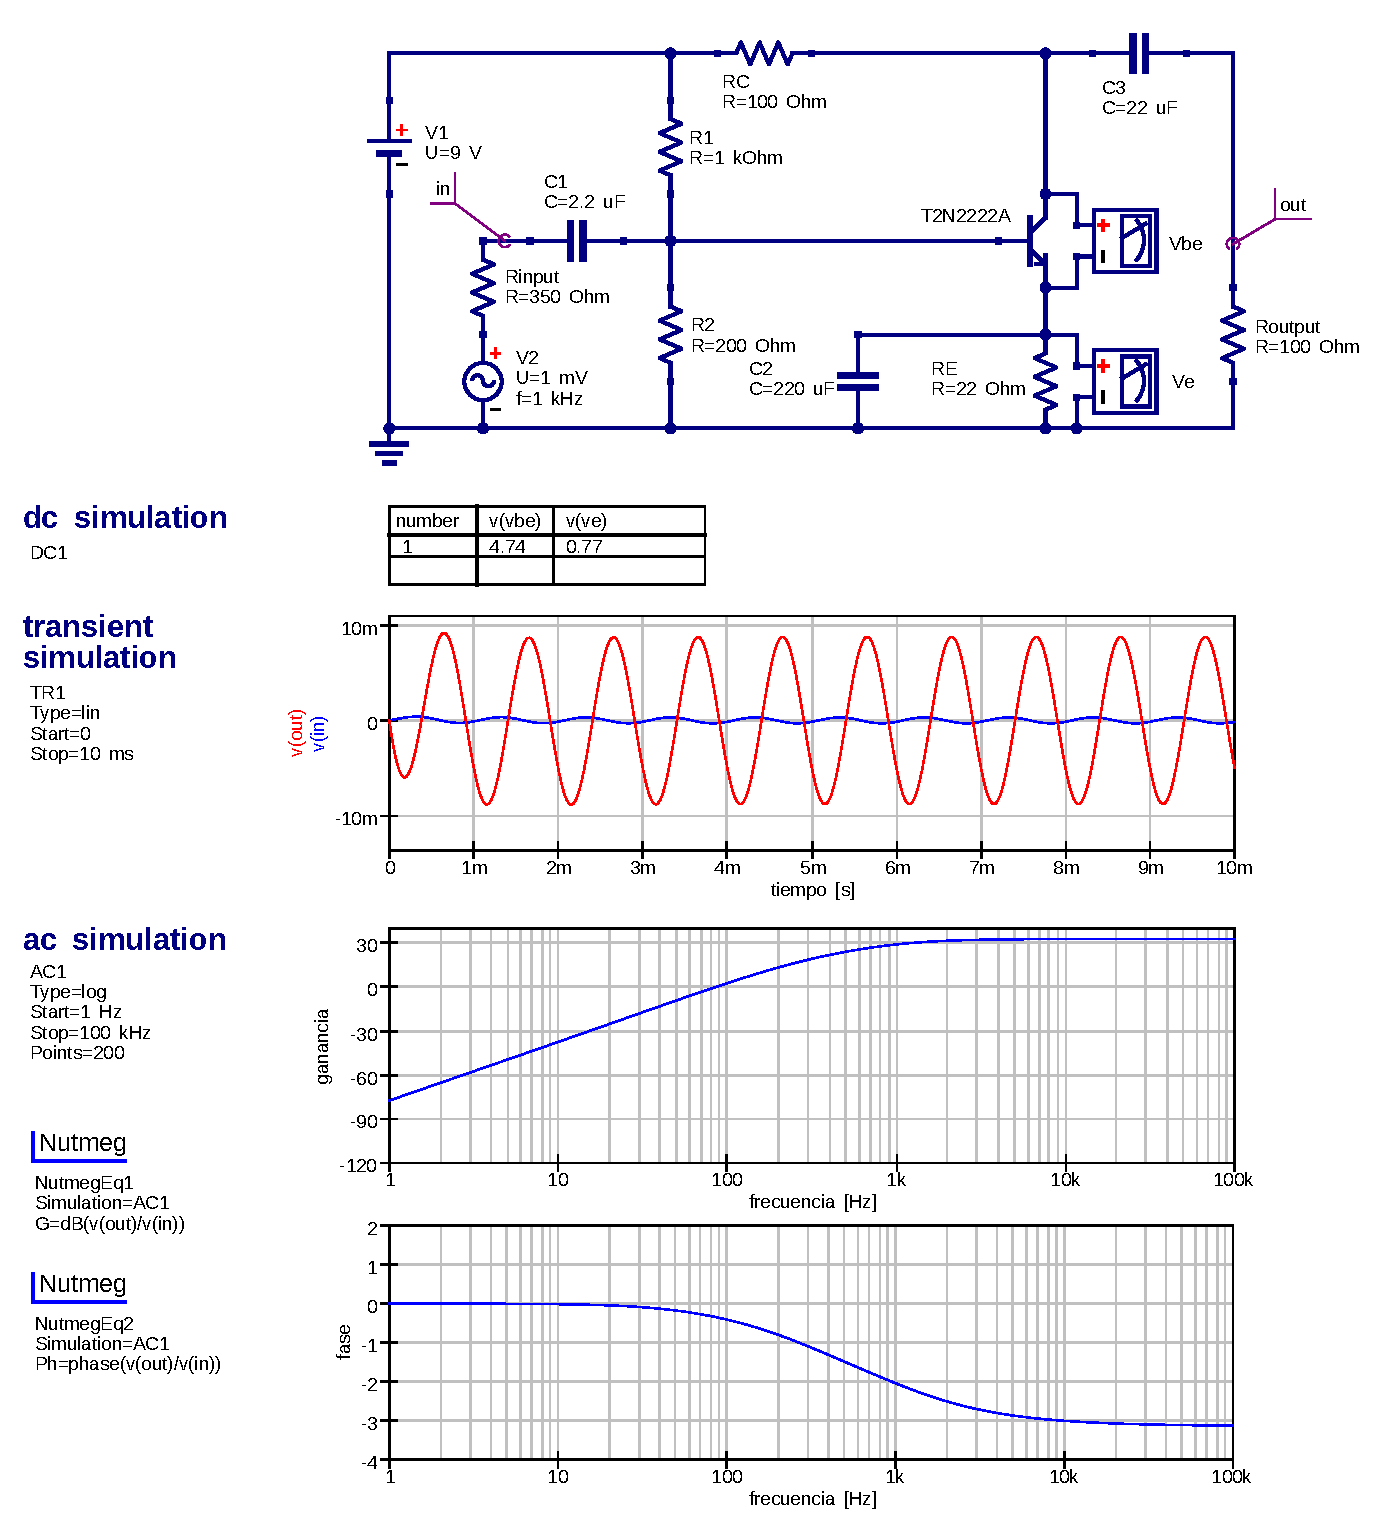
\includegraphics[scale=0.72]{diagramas/figura23.eps}
\caption{Simulación del amplificador.}
\label{figura23}
\end{figure}

